\section{Lab 1} 

\subsection{Introduction} \label{sec:Introduction}

This report presents the development of an electropneumatic control system inspired by the 
setup "P3. EPM-TWD-2.3." The objective is to design a functional control scheme that can be
utilized for automation processes such as elevators, conveyor belts, or doors. The control system 
integrates fundamental electropneumatic components, including double-action and single-action cylinders, 
valves, buttons, and sensors, ensuring a comprehensive understanding of industrial automation.

The system considers electric push buttons B1 and B2, along with electric limit switches I7 
and I8, which are simulated using pneumatic 3/2 valves. Additionally, an electric switch button 
B3 commands a unique solenoid valve SV1, playing a crucial role in the automation process. A 
pneumatic 3/2 valve with a manual control (B0) is also incorporated to regulate airflow from the 
compressor. Different valve command methods—manual, mechanical, pneumatic, and electropneumatic—are 
explored to enhance system flexibility.

Beyond the core components, additional elements such as logic valves (AND, OR, NOT), a bistable
 memory-type valve, flow control valves, and an on-delay NC pneumatic timer are included to optimize 
 system efficiency. The inclusion of extra cylinders, more valves, pneumatic-electrical converters, a 
 lamp, and a buzzer further enhances functionality.

The report systematically covers the design, implementation, and simulation of the control system 
using Fluidism 3.6 software. The following sections outline the schematic design, control loop 
architecture, automation specifications, Grafcet representation, and simulation results.

\subsection{Process Schematic and Sensor-Actuator Integration} \label{sec:Process_Schematic_and_Sensor-Actuator_Integration}

The first step in the system design is to create a schematic representation of the process, 
illustrating the placement of sensors and actuators. This diagram serves as a foundational blueprint 
for the entire control system. The schematic includes the necessary cylinders, valves, and control 
components to facilitate automation.

\begin{figure}[H]
    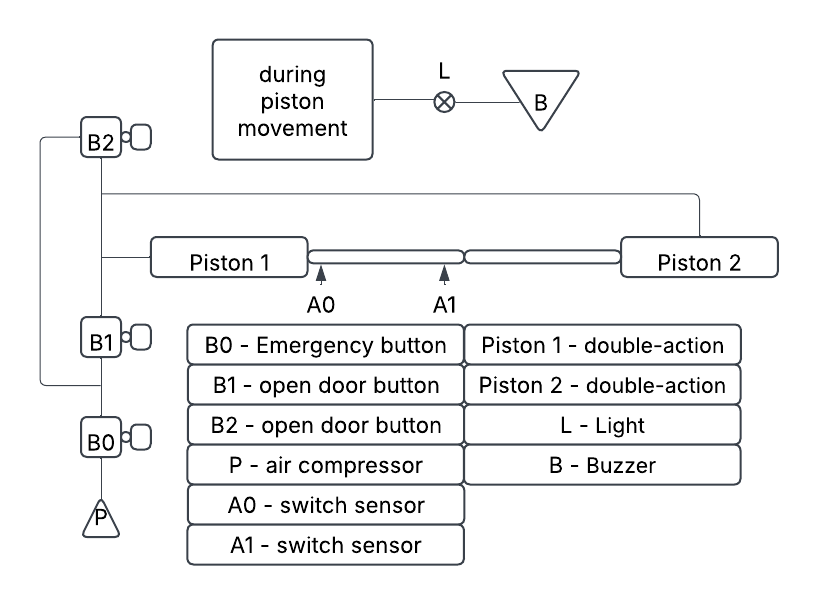
\includegraphics[width=16cm]{Images/schematic.png}
    \centering
    \caption{Decided schematic for the door control}
    \label{fig:schematic}
\end{figure}

This schematic\ref{fig:schematic} illustrates the design of a double-cylinder door mechanism. Both Buttons B1 and B2 
can be used to open the door, which remains open for approximately five seconds after the button is 
released. Additionally, two emergency buttons (B3 and B0) are included—one pneumatic and the other 
electropneumatic—to disconnect the compressor in case of an emergency.

\subsection{Control Loop Architecture} \label{sec:Control_Loop_Architecture}

The control loop architecture is a critical component of the automation process. It 
defines the relationship between controllers, actuators, processes, and sensors. By 
analyzing the control loop, we ensure the seamless execution of the automation cycle while maintaining safety and efficiency.

\begin{figure}[H]
    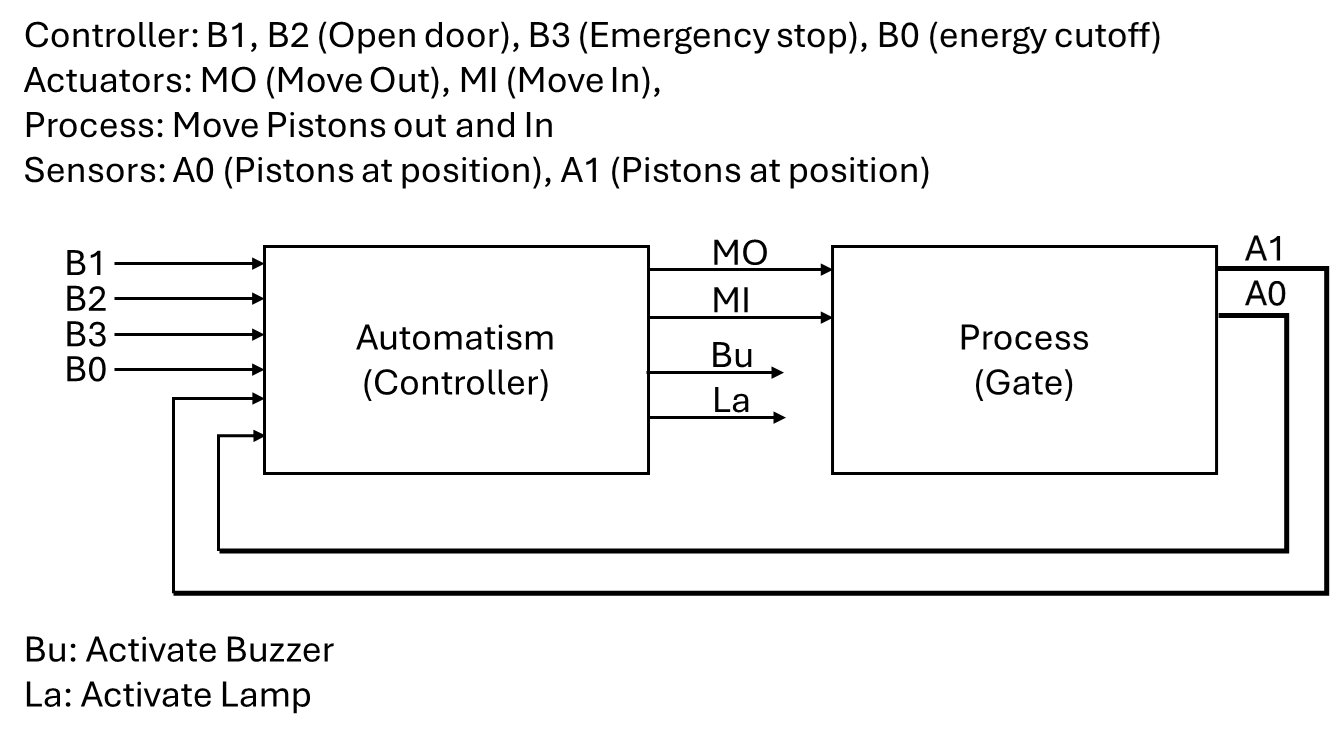
\includegraphics[width=16cm]{Images/control_loop.png}
    \centering
    \caption{Control loop for the door control}
    \label{fig:control_loop}
\end{figure}

The control loop schematic\ref{fig:control_loop} outlines the automation process, which operates using four buttons. 
The outputs control the motion of the door cylinders—retracting (MI) and extending (MO). 
A lamp and a buzzer provide visual and auditory feedback on the cylinders' movement. Sensors 
A0 and A1 detect whether the cylinder is fully opened or closed, ensuring accurate control of the system.

\subsection{Automation Specifications} \label{sec:Automation_Specifications}

To ensure the effectiveness of the designed system, various types of automation 
specifications are described. These specifications include operational conditions, 
safety requirements, timing constraints, and failure handling procedures.

Working Specifications:
\begin{itemize}
    \item The button B0 halts all movement, button B3 disables pressure source.
    \item Buttons B1 and B2 trigger the opening of the gate; Cylinders move towards A0 (MI). 
    Can only be pressed if Cylinders are at positions A0 or A1.
    \item If gate is open (Cyl at A0),  wait 5 seconds before closing gate (MO).
    \item While cylinders are moving, activate Buzzers (Bu) and Lamps (La).
    \item Pressure is 6 bar, voltage is 24V.
\end{itemize}

\subsection{Grafcet Representation} \label{sec:Grafcet_Representation}

A structured graphical representation of the automation sequence is developed using the 
Grafcet method. This step-by-step graphical model illustrates the transitions between 
different states of the system, ensuring a clear understanding of the control logic.

\begin{figure}[H]
    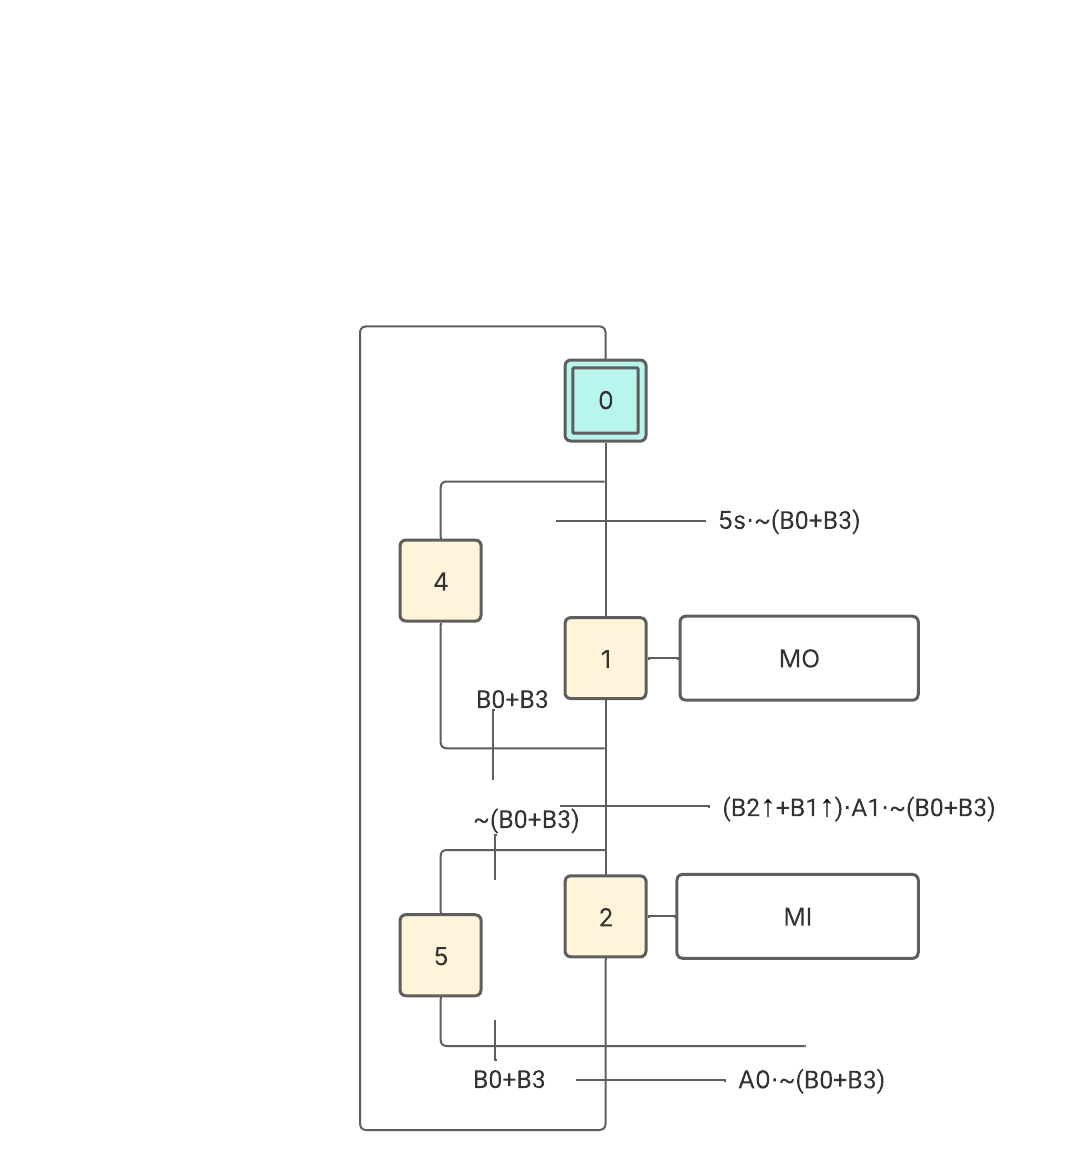
\includegraphics[width=16cm]{Images/grafset.png}
    \centering
    \caption{Grafset for the door control}
    \label{fig:grafset}
\end{figure}

The Grafcet diagram presents a structured graphical representation of the automation sequence. It clearly defines 
the different states and transitions of the system, offering an intuitive 
understanding of how the automation logic operates based on the control loop described in Section \ref{sec:Control_Loop_Architecture}.

\subsection{Simulation and Validation} \label{sec:Simulation_and_Validation}

The final stage involves simulating the closed-loop control system in Fluidism 3.6 software. 
The simulation tests the interaction between the automation process, sensors, and actuators, 
validating whether the system meets the defined specifications. Any deviations are analyzed, 
and necessary modifications are proposed to optimize system performance.

\begin{figure}[H]
    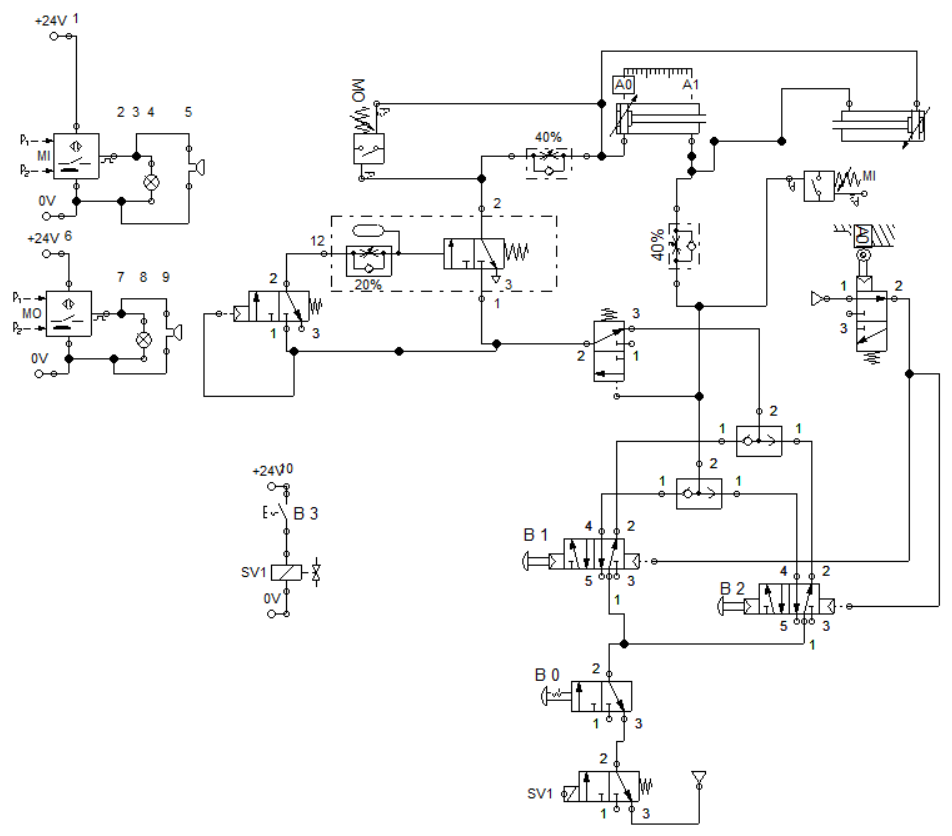
\includegraphics[width=16cm]{Images/fluidsim.png}
    \centering
    \caption{Fluidsim for the door control}
    \label{fig:fluidsim}
\end{figure}

The complete implementation of the control system in FluidSim 3.6 is shown here. The design includes two OR gates, 
allowing both control buttons to be used as needed. The emergency buttons (one pneumatic and one electropneumatic) 
are also visible. Due to software constraints, the circuit controlling the light and buzzer had to be duplicated, as 
each pneumatic-to-electrical converter could only be connected to a single differential pressure switch—one for the 
opening motion and another for closing.\\

Do take care that the circuit made to control the light and buzzer had to be duplicated in simulation 
since for each pneumatic to eletrical converted could only be conected to one differential pressure switch, 2 were necessary
one for the opening motion and one for the closing.

\subsection{Conclusion}

This report details the complete development of an electropneumatic control system, from schematic 
design to simulation validation. By integrating various automation components and methodologies, 
the system achieves a robust and efficient control mechanism. The findings highlight the importance 
of precise component selection and control logic design in achieving a functional and reliable 
automated process.